\documentclass[12pt,a4paper]{report}
\usepackage[left=1.25in,right=1in,top=0.75in,bottom=0.75in]{geometry}
\usepackage{mathptmx} % Times New Roman font
\usepackage{setspace}
\usepackage{graphicx}
\usepackage{titlesec}
\usepackage{tocloft}
\usepackage{indentfirst} % Indent first paragraph
\usepackage{xcolor}
\usepackage{tikz}
\usepackage{pgfplots}
\pgfplotsset{compat=1.18}
\usetikzlibrary{shapes.geometric, arrows.meta, positioning, calc, patterns, fit}

\onehalfspacing % 1.5 line spacing

% --- Formatting Chapters ---
\titleformat{\chapter}[display]
  {\normalfont\bfseries}
  {\fontsize{16pt}{19.2pt}\selectfont\raggedright Chapter \thechapter} % Chapter number left justified, font size 16 bold
  {1ex}
  {\fontsize{18pt}{21.6pt}\selectfont\centering} % Chapter title centered, font size 18 bold

\titlespacing*{\chapter}{0pt}{-20pt}{20pt} % Adjust top spacing for chapters

% --- Formatting Sections ---
\titleformat{\section}
  {\normalfont\fontsize{14pt}{16.8pt}\bfseries\raggedright} % Section left justified, font size 14 bold
  {\thesection}{1em}{}

% --- Formatting Subsections ---
\titleformat{\subsection}
  {\normalfont\fontsize{12pt}{14.4pt}\bfseries\raggedright} % Subsection left justified, font size 12 bold
  {\thesubsection}{1em}{}

% Table of Contents customizations to match the provided layout
\renewcommand{\cftchapfont}{\normalfont\fontsize{12pt}{14.4pt}\selectfont}
\renewcommand{\cftchappagefont}{\normalfont\fontsize{12pt}{14.4pt}\selectfont}
\renewcommand{\cftchapleader}{\cftdotfill{\cftdotsep}}

\begin{document}

% ==========================================
% COVER PAGE
% ==========================================
\begin{titlepage}
\begin{center}
\textbf{\Large Project Progress Report on}

\vspace{0.3cm}
\hrule height 2pt
\vspace{0.15cm}
\hrule height 1pt
\vspace{0.5cm}
\textbf{\Large SECUREBANK: A HYBRID STATISTICAL AND NEURAL NETWORK FRAMEWORK FOR CONTINUOUS BEHAVIORAL AUTHENTICATION ON MOBILE BANKING PLATFORMS}
\vspace{0.4cm}
\hrule height 1pt
\vspace{0.15cm}
\hrule height 2pt

\vspace{0.8cm}
\textbf{Submitted in partial fulfilment of the requirement for the award of the degree of}

\vspace{0.6cm}
\textbf{BACHELOR OF TECHNOLOGY}

\vspace{0.3cm}
\textbf{IN}

\vspace{0.3cm}
\textbf{COMPUTER SCIENCE \& ENGINEERING}

\vspace{0.5cm}
\textbf{Submitted by:}
\end{center}

\vspace{0.2cm}
\begin{table}[h]
\centering
\bfseries
\renewcommand{\arraystretch}{1.5}
\begin{tabular}{ll}
Tejus Kapoor     & University Roll No. [Roll No] \\
Tanush Malhotra  & University Roll No. [Roll No] \\
Bela Diwan       & University Roll No. [Roll No] \\
Gautam Nautiyal  & University Roll No. [Roll No] \\
\end{tabular}
\end{table}

\begin{center}
\vspace{0.5cm}
\textit{Under the Guidance of}\\
\textbf{[Guide Name]}\\
\textbf{[Designation]}

\vspace{0.8cm}
\textbf{Project Team ID: [ID No.]}\\
\vspace{0.4cm}
\textbf{Project Progress Report No: 1}

\vspace{1.0cm}

\includegraphics[width=4cm]{geu_logo.jpg} 

\vspace{1.0cm}
\textbf{\Large Department of Computer Science and Engineering}\\
\textbf{\Large Graphic Era (Deemed to be University)}\\
\textbf{\Large Dehradun, Uttarakhand}\\
\textbf{\Large 2025-26}
\end{center}
\end{titlepage}

% ==========================================
% CANDIDATE'S DECLARATION
% ==========================================
\newpage
\thispagestyle{empty}
\begin{center}

\includegraphics[width=5cm]{geu_logo.jpg}
\vspace*{0.5cm}
\textbf{\Large CANDIDATE'S DECLARATION}
\end{center}
\vspace{0.5cm}

\noindent I/We hereby certify that the work which is being presented in the project progress report entitled \textbf{``SecureBank: A Hybrid Statistical and Neural Network Framework for Continuous Behavioral Authentication on Mobile Banking Platforms''} in partial fulfillment of the requirements for the award of the Degree of Bachelor of Technology in Computer Science and Engineering in the Department of Computer Science and Engineering of the Graphic Era (Deemed to be University), Dehradun shall be carried out by the undersigned under the supervision of \textbf{[Guide Name], [Designation]}, Department of Computer Science and Engineering, Graphic Era (Deemed to be University), Dehradun.

\vspace{1.2cm}
\begin{table}[h]
\centering
\renewcommand{\arraystretch}{1.5}
\begin{tabular}{p{0.35\textwidth} p{0.35\textwidth} p{0.25\textwidth}}
Tejus Kapoor & University Roll No. [Roll No] & \textcolor{gray}{\textit{signature}} \\
Tanush Malhotra & University Roll No. [Roll No] & \textcolor{gray}{\textit{signature}} \\
Bela Diwan & University Roll No. [Roll No] & \textcolor{gray}{\textit{signature}} \\
Gautam Nautiyal & University Roll No. [Roll No] & \textcolor{gray}{\textit{signature}} \\
\end{tabular}
\end{table}

\vspace{1.0cm}
\begin{center}
The above mentioned students shall be working under the supervision of the undersigned on the \textbf{``SecureBank: A Hybrid Statistical and Neural Network Framework for Continuous Behavioral Authentication on Mobile Banking Platforms''}
\end{center}

\vspace{1.5cm}
\noindent \textbf{Supervisor} \hfill \textbf{Head of the Department}

\vspace{1.5cm}
\begin{center}
\textbf{\underline{Examination}}
\end{center}

\vspace{1.0cm}
\noindent \textbf{Name of the Examiners:} \hfill \textbf{Signature with Date}

\vspace{0.5cm}
\noindent 1. 

\vspace{0.5cm}
\noindent 2.
\newpage

% ==========================================
% TABLE OF CONTENTS
% ==========================================
\pagenumbering{roman}
\renewcommand{\contentsname}{\begin{center}\textbf{\Large Table of Contents}\end{center}\vspace{-1cm}}
\tableofcontents
\newpage

\pagenumbering{arabic}

% ==========================================
% CHAPTER 1: INTRODUCTION AND PROBLEM STATEMENT
% ==========================================
\chapter{Introduction and Problem Statement}

In the following sections, a brief introduction and the problem statement for the work has been included.

\section{Introduction}

Most banking applications on Android stop verifying the user's identity the moment they successfully log in. A single checkpoint---such as a PIN, fingerprint, or password---is typically all that prevents unauthorized access. Consequently, if an authorized session is left unattended, any individual possessing the device gains complete access to sensitive financial functions, and the application remains oblivious to the transition.

In response to the increasing threat of unauthorized mobile transactions and mobile banking fraud, behavioral biometrics has emerged as a promising continuous authentication solution. This concept leverages the unique ways in which individuals interact with their devices, including typing rhythms, touch patterns, and phone-holding postures, to continuously and reliably verify their identity invisibly.

The present work introduces \textit{SecureBank}, an Android application prototype that directly addresses this specific vulnerability. It continuously observes how a user interacts with the mobile device post-login by monitoring keystrokes (such as PIN pad entry timings), touch events (taps, swipes, durations, and pressures), and movement vectors from on-board sensors (accelerometer and gyroscope). 

The detailed architectural framework incorporates a hybrid engine that evaluates behavioral drift. A statistical Z-score track detects rapid and obvious deviations from login baselines, functioning alongside a machine learning track powered by an on-device Multi-Layer Perceptron (MLP) neural network. These combined analytics enable SecureBank to calculate accurate risk indicators in real-time without negatively impacting the device’s efficiency or battery life.

\section{Problem Statement}

The problem statement for the present work can be stated as follows:

To develop and evaluate a continuous, non-intrusive behavioral authentication system for mobile banking applications capable of silently observing post-login user activities, including keystroke dynamics, touchscreen interactions, and device holding motion metrics. The system must employ a localized hybrid risk detection engine—fusing statistical Z-score approximations with an efficient on-device Multi-Layer Perceptron (MLP) neural network—to accurately translate measured behavioral deviations into real-time risk scores. Based on these computed safety metrics, the framework must systematically orchestrate corresponding security responses, such as displaying cautionary warnings, issuing re-authentication demands, or enforcing immediate forced logouts, to preclude unauthorized access during an active session in the event of device abandonment or interception.

% ==========================================
% CHAPTER 2: OBJECTIVES
% ==========================================
\chapter{Objectives}

The proposed work objectives are as follows:

\begin{itemize}
    \item \textbf{Develop an Android-based continuous authentication prototype:} To design and build a native Android banking application capable of silently gathering keystroke timings, touchscreen dynamics, and inertial motion data in the background without affecting performance or battery consumption.
    \item \textbf{Formulate an enrollment-relative feature engineering pipeline:} To convert raw sensor inputs into stable baseline-relative deviation features, quantifying behavioral drifts precisely starting from the initial PIN entry.
    \item \textbf{Implement an on-device hybrid detection algorithm:} To construct a dual-track security monitoring engine integrating statistical Z-scores with a compiled lightweight Multi-Layer Perceptron (MLP) model utilizing highly-efficient matrix mathematics inside the Kotlin environment.
    \item \textbf{Evaluate multi-feature importance and system precision:} To analyze performance statistics on synthetic and real behavioral datasets under 5-fold cross-validation, and establish which characteristics (e.g., motion relative deviations versus keystroke durations) contribute most successfully to distinguishing impostors from authentic operators.
    \item \textbf{Enforce adaptive, graduated security interventions:} To automatically map aggregated anomaly scores to varying response protocols including passive continuations, soft warnings, re-authentication demands, and immediate session terminations based upon measured risk thresholds.
\end{itemize}

% ==========================================
% CHAPTER 3: PROJECT WORK CARRIED OUT
% ==========================================
\chapter{Project Work Carried Out}

The development of the continuous behavioral authentication framework involved several distinct phases of engineering and research. The primary work carried out to date includes:

\begin{itemize}
    \item \textbf{System Architecture \& UI Integration:} Developed the core Android application using Jetpack Compose and Kotlin Coroutines, adhering to an MVVM (Model-View-ViewModel) logic separation for maintainability and efficient state management.
    \item \textbf{Sensor Array Collection Mechanisms:} Successfully implemented background listeners to systematically gather multi-modal inputs. This includes a custom numerical PIN-pad for high-resolution keystroke capture, pointer interceptors for touchscreen gestures, and moving-average filters for smoothing raw accelerometer and gyroscope hardware signals.
    \item \textbf{Data Persistence Layer:} Integrated a localized Room SQLite database to temporarily buffer structured telemetry sequences, ensuring robust real-time availability without relying on cloud transmissions and preserving privacy.
    \item \textbf{Feature Engineering Pipeline:} Finalized the algorithms computing the 124-dimensional deviation vectors, ensuring the system calculates drift relatively against the genuine user's initial login signatures rather than evaluating absolute raw values.
    \item \textbf{Model Execution \& Deployment:} Engineered a synthetic data generator script in Python to expand the limited physical trial subset. Successfully trained a lightweight Multi-Layer Perceptron (MLP) neural network and deployed its JSON weights iteratively directly into the Kotlin environment, averting the footprint overhead of external libraries.
\end{itemize}

\vspace{0.5cm}
\begin{figure}[htbp]
\centering
\resizebox{0.75\textwidth}{!}{%
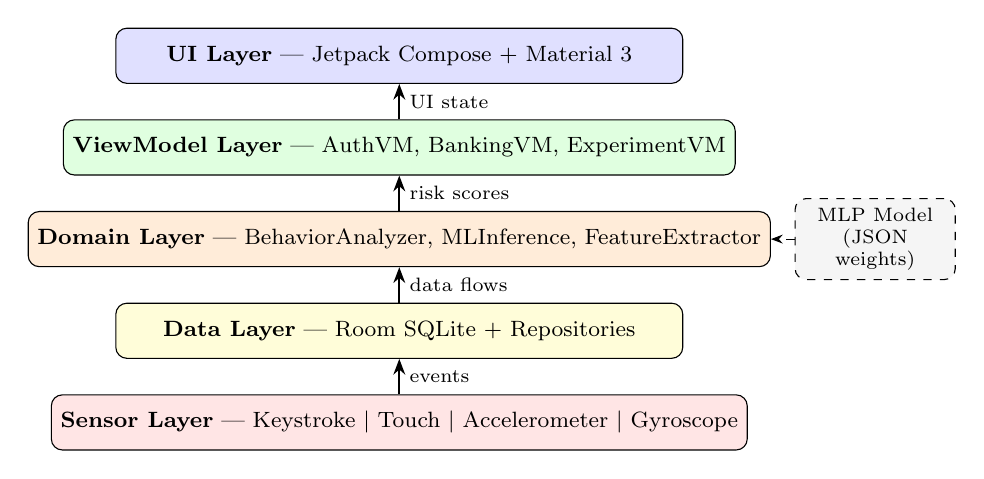
\begin{tikzpicture}[
    layer/.style={draw, rounded corners, minimum width=7.2cm, minimum height=0.7cm, align=center, font=\footnotesize},
    arrow/.style={-{Stealth[length=2mm]}, thick},
    node distance=0.45cm
]
\node[layer, fill=blue!12] (ui) {\textbf{UI Layer} --- Jetpack Compose + Material 3};
\node[layer, fill=green!12, below=of ui] (vm) {\textbf{ViewModel Layer} --- AuthVM, BankingVM, ExperimentVM};
\node[layer, fill=orange!15, below=of vm] (domain) {\textbf{Domain Layer} --- BehaviorAnalyzer, MLInference, FeatureExtractor};
\node[layer, fill=yellow!15, below=of domain] (data) {\textbf{Data Layer} --- Room SQLite + Repositories};
\node[layer, fill=red!10, below=of data] (sensor) {\textbf{Sensor Layer} --- Keystroke $\vert$ Touch $\vert$ Accelerometer $\vert$ Gyroscope};

\draw[arrow] (sensor) -- node[right, font=\scriptsize] {events} (data);
\draw[arrow] (data) -- node[right, font=\scriptsize] {data flows} (domain);
\draw[arrow] (domain) -- node[right, font=\scriptsize] {risk scores} (vm);
\draw[arrow] (vm) -- node[right, font=\scriptsize] {UI state} (ui);

\node[draw, dashed, rounded corners, fill=gray!8, font=\scriptsize, text width=1.8cm, align=center, right=0.3cm of domain] (ml) {MLP Model\\(JSON weights)};
\draw[-{Stealth[length=1.5mm]}, dashed] (ml) -- (domain);

\end{tikzpicture}%
}
\caption{Layered architecture of SecureBank demonstrating the flow of behavioral data.}
\label{fig:architecture}
\end{figure}

\vspace{0.5cm}
\begin{figure}[htbp]
\centering
\resizebox{0.75\textwidth}{!}{%
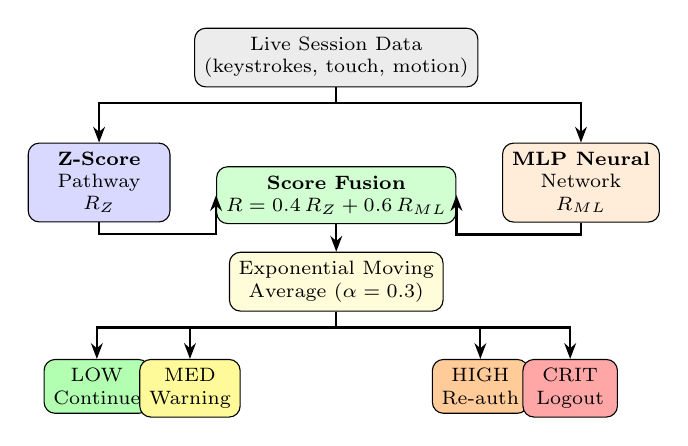
\begin{tikzpicture}[
    box/.style={draw, rounded corners, minimum height=0.6cm, align=center, font=\scriptsize},
    decision/.style={draw, diamond, aspect=2, inner sep=1pt, font=\scriptsize, align=center},
    arrow/.style={-{Stealth[length=2mm]}, thick},
    node distance=0.4cm and 0.3cm
]
\node[box, fill=gray!15, minimum width=2.2cm] (input) {Live Session Data\\(keystrokes, touch, motion)};

\node[box, fill=blue!15, below left=0.7cm and 0.3cm of input, minimum width=1.8cm] (zscore) {\textbf{Z-Score}\\Pathway\\$R_Z$};
\node[box, fill=orange!15, below right=0.7cm and 0.3cm of input, minimum width=1.8cm] (mlpath) {\textbf{MLP Neural}\\Network\\$R_{\text{ML}}$};

\draw[arrow] (input.south) -- ++(0,-0.2) -| (zscore.north);
\draw[arrow] (input.south) -- ++(0,-0.2) -| (mlpath.north);

\node[box, fill=green!18, below=1.0cm of input, minimum width=2.2cm] (fusion) {\textbf{Score Fusion}\\$R = 0.4\,R_Z + 0.6\,R_{\text{ML}}$};
\draw[arrow] (zscore.south) -- ++(0,-0.15) -| (fusion.west);
\draw[arrow] (mlpath.south) -- ++(0,-0.15) -| (fusion.east);

\node[box, fill=yellow!15, below=0.35cm of fusion, minimum width=2.2cm] (ema) {Exponential Moving\\Average ($\alpha=0.3$)};
\draw[arrow] (fusion) -- (ema);

\node[box, fill=green!30, below left=0.6cm and 1.0cm of ema, minimum width=1.2cm] (low) {LOW\\Continue};
\node[box, fill=yellow!40, below left=0.6cm and -0.15cm of ema, minimum width=1.2cm] (med) {MED\\Warning};
\node[box, fill=orange!40, below right=0.6cm and -0.15cm of ema, minimum width=1.2cm] (high) {HIGH\\Re-auth};
\node[box, fill=red!35, below right=0.6cm and 1.0cm of ema, minimum width=1.2cm] (crit) {CRIT\\Logout};

\draw[arrow] (ema.south) -- ++(0,-0.2) -| (low.north);
\draw[arrow] (ema.south) -- ++(0,-0.2) -| (med.north);
\draw[arrow] (ema.south) -- ++(0,-0.2) -| (high.north);
\draw[arrow] (ema.south) -- ++(0,-0.2) -| (crit.north);

\end{tikzpicture}%
}
\caption{The hybrid detection pipeline integrating Z-score and Neural Network predictions.}
\label{fig:hybrid}
\end{figure}

% ==========================================
% CHAPTER 4: FUTURE WORK PLAN
% ==========================================
\chapter{Future Work Plan}

Moving forward, the project roadmap includes several enhancements aimed at refining the security model and optimizing user interactions:

\begin{enumerate}
    \item \textbf{Large-Scale Real User Study:} Organize an extensive data gathering phase with over 30 physical participants to completely replace synthetic data paradigms, validating the model's generalized reliability across diverse demographics.
    \item \textbf{Implementation of Adaptive Baselines:} Develop logic allowing the baseline profile to silently and progressively drift alongside the user's naturally evolving grip habits or typing cadences, minimizing false rejections over long deployments.
    \item \textbf{Exploration of Temporal Sequence Models:} Investigate complex sequence-based machine learning structures, such as LSTMs (Long Short-Term Memory networks) or Transformers, to directly assess chronological behavioral patterns rather than statistically aggregated timeframes.
    \item \textbf{Deep Operating System Interventions:} Hook the warning triggers directly into Android's native \texttt{BiometricPrompt} frameworks, granting frictionless fingerprint or facial re-authentication instead of enforcing hard logouts during borderline risk evaluations.
\end{enumerate}

% ==========================================
% CHAPTER 5: WEEKLY TASK
% ==========================================
\chapter{Weekly Task}

The following timeline details the weekly milestones accomplished throughout the continuous development of this major project:

\begin{itemize}
    \item \textbf{Week 1 -- 2:} Comprehensive literature review concerning continuous mobile authentication; initial project scoping, requirement gathering, and MVVM architectural planning.
    \item \textbf{Week 3 -- 4:} Implementation of the custom Android keystroke, touch, and localized motion hardware sensor collectors within background services.
    \item \textbf{Week 5 -- 6:} Setting up the local Room structured database, testing data ingestion logic, and recording preliminary data from pilot participants.
    \item \textbf{Week 7 -- 8:} Python-based synthetic data augmentation setup; devising the feature engineering mathematical structures leading to the computation of 124-dimensional deviation arrays.
    \item \textbf{Week 9 -- 10:} Extensive model training comparing Random Forest, Support Vector Machines, and Multi-Layer Perceptrons. Translation of the preferred MLP weights into portable JSON formatting.
    \item \textbf{Week 11 -- 12:} Development of the on-device customized Kotlin matrix multiplication inference engine, alongside the synchronized statistical Z-score pathway and integrated risk-level mapping.
    \item \textbf{Week 13 -- 14:} Comprehensive end-to-end system testing, 5-fold cross-validation computational evaluation, and composing the initial project progress documentation.
\end{itemize}

% ==========================================
% REFERENCES
% ==========================================
\renewcommand{\bibname}{References}
\begin{thebibliography}{9}

\bibitem{ecb2022}
European Central Bank, ``Fifth report on card fraud,'' \textit{ECB Statistical Paper Series}, 2022.

\bibitem{killourhy2009}
K.~S.~Killourhy and R.~A.~Maxion, ``Comparing anomaly-detection algorithms for keystroke dynamics,'' in \textit{Proc. IEEE/IFIP Int. Conf. Dependable Systems \& Networks (DSN)}, 2009, pp. 125--134.

\bibitem{frank2013}
M.~Frank, R.~Biedert, E.~Ma, I.~Martinovic, and D.~Song, ``Touchalytics: On the applicability of touchscreen input as a behavioral biometric for continuous authentication,'' \textit{IEEE Trans. Inf. Forensics Security}, vol.~8, no.~1, pp. 136--148, Jan. 2013.

\bibitem{sitova2016}
Z.~Sitov\'{a} et~al., ``HMOG: New behavioral biometric features for continuous authentication of smartphone users,'' \textit{IEEE Trans. Inf. Forensics Security}, vol.~11, no.~5, pp. 877--892, May 2016.

\end{thebibliography}

\end{document}
